\chapter{उत्प्रेरण}\label{ch:g12:catalysis}

हाइड्रोजन परॉक्साइड विलयन की एक बोतल बाथरूम की अलमारी में महीनों तक
बिना बदले पड़ी रहती है। छिले हुए घुटने पर डालते ही वह तुरंत झाग देने लगता है:
रक्त में मौजूद कोई चीज़ उसे सेकंडों में पानी और ऑक्सीजन में
अपघटित कर देती है। वह चीज़ खपती नहीं, और अभिक्रिया के समीकरण में
दिखाई नहीं देती। वह एक \omterm{def:g12:catalysis:catalyst}{उत्प्रेरक} है। \omterm{def:g12:catalysis:catalyst}{उत्प्रेरक} ही अधिकांश
रासायनिक उद्योग को संभव बनाते हैं, कारों के धुएँ को साफ़ करते हैं, और जीवन की हर
अभिक्रिया चलाते हैं।

\begin{recall}
किसी अभिक्रिया की दर और उसे बदलने वाले \omterm{def:g12:reaction-rates:kinetic-factor}{गतिक कारक}
(\cref{ch:g12:reaction-rates})। क्रियाविधि \omterm{def:g12:curly-arrows:mechanism}{मूल चरणों} की एक श्रृंखला है,
जो मध्यवर्तियों से होकर गुज़रती है (\cref{ch:g12:curly-arrows})।
\end{recall}

\section{उत्प्रेरक क्या है}

\begin{definition}[उत्प्रेरक, उत्प्रेरण]\label{def:g12:catalysis:catalyst}
\emph{उत्प्रेरक}\index{उत्प्रेरक} वह स्पीशीज़ है जो किसी अभिक्रिया को
बिना खपे तेज़ कर देती है: वह क्रियाविधि में भाग लेती है पर अंत में
अपरिवर्तित वापस मिल जाती है, और समग्र समीकरण में दिखाई नहीं
देती। उत्प्रेरक द्वारा किसी अभिक्रिया का तेज़ होना
\emph{उत्प्रेरण}\index{उत्प्रेरण} है।
\end{definition}

\begin{proposition}[उत्प्रेरक रास्ता बदलता है, मंज़िल नहीं]\label{prop:g12:catalysis:path}
\omterm{def:g12:catalysis:catalyst}{उत्प्रेरक} एक भिन्न क्रियाविधि खोलता है, जिसकी ऊर्जा बाधाएँ
अनुत्प्रेरित अभिक्रिया की बाधा से कम होती हैं, जिससे कणों के बीच के अधिक
मिलन सफल होते हैं। वह न बनने वाले उत्पादों को बदलता है, न
पहुँची गई \omterm{def:g10:reaction-progress-table:system}{अंतिम अवस्था} को; वह केवल उस तक जल्दी पहुँचाता है।
\end{proposition}

\begin{proof}
स्वीकृत: ऊर्जा-रूपरेखा का अध्ययन विश्वविद्यालय के प्रथम वर्ष के खंड में है। यह कि \omterm{def:g10:reaction-progress-table:system}{अंतिम
अवस्था} नहीं बदलती, \omterm{def:g12:catalysis:catalyst}{उत्प्रेरक} के वापस मिलने से निकलता है:
समग्र अभिक्रिया, \omterm{def:g7:chemical-reactions:reactant}{अभिकारक} और उत्पाद, वही रहती है।
\end{proof}

\begin{omfigure}
\begin{minipage}{0.49\linewidth}
\begin{tikzpicture}
\begin{axis}[width=\linewidth, height=5.4cm, xmin=0, xmax=1, ymin=-60,
    ymax=110, xtick=\empty, ytick=\empty, axis lines*=left,
    xlabel={अभिक्रिया की प्रगति}, ylabel={ऊर्जा},
    label style={font=\small}, legend style={font=\scriptsize,
    at={(0.02,0.99)}, anchor=north west, draw=none}, legend cell align=left]
  \addplot[very thick, omDef] table[x=s, y=Eu] {figdata/out/grade-12-catalysis-a.dat};
  \addplot[very thick, omProp] table[x=s, y=Ec] {figdata/out/grade-12-catalysis-a.dat};
  \legend{उत्प्रेरक के बिना, उत्प्रेरक के साथ}
  \node[font=\scriptsize, anchor=north west] at (axis cs:0.02,-4) {अभिकारक};
  \node[font=\scriptsize, anchor=south east] at (axis cs:0.99,-36) {उत्पाद};
\end{axis}
\end{tikzpicture}
\end{minipage}\hfill
\begin{minipage}{0.49\linewidth}
\begin{tikzpicture}
\begin{axis}[width=\linewidth, height=5.4cm, xmin=0, xmax=60, ymin=0,
    ymax=80, xlabel={$t$ (\si{min})}, ylabel={निकली \ce{O2} (\si{mL})},
    axis lines*=left, ymajorgrids, grid style={gray!20},
    tick label style={font=\scriptsize}, label style={font=\small},
    legend style={font=\scriptsize, at={(0.98,0.03)}, anchor=south east,
    draw=none}, legend cell align=left]
  \addplot[very thick, omDef] table[x=t, y=Vu] {figdata/out/grade-12-catalysis-b.dat};
  \addplot[very thick, omProp] table[x=t, y=Vc] {figdata/out/grade-12-catalysis-b.dat};
  \legend{उत्प्रेरक के बिना, उत्प्रेरक के साथ}
\end{axis}
\end{tikzpicture}
\end{minipage}

{\small बाएँ: अभिक्रिया के साथ ऊर्जा; उत्प्रेरित रास्ता
एक मध्यवर्ती और दो निचली बाधाओं से होकर जाता है। दाएँ: हाइड्रोजन परॉक्साइड
विलयन से निकली ऑक्सीजन; \omterm{def:g12:catalysis:catalyst}{उत्प्रेरक} अभिक्रिया को तेज़ करता है, पर
अंतिम आयतन वही रहता है। (मॉडल वक्र।)}
\end{omfigure}

\section{समांगी उत्प्रेरण}

\begin{definition}[समांगी और विषमांगी उत्प्रेरण]\label{def:g12:catalysis:homogeneous}
\omterm{def:g12:catalysis:catalyst}{उत्प्रेरण} \emph{समांगी उत्प्रेरण}\index{समांगी उत्प्रेरण} है
जब \omterm{def:g12:catalysis:catalyst}{उत्प्रेरक} \omterm{def:g7:chemical-reactions:reactant}{अभिकारकों} वाली प्रावस्था में ही हो (उदाहरण के लिए
उनके साथ घुला हुआ), और \emph{विषमांगी उत्प्रेरण}\index{विषमांगी उत्प्रेरण}
जब वह किसी दूसरी प्रावस्था में हो, आम तौर पर एक ठोस जिसकी सतह तक
\omterm{def:g7:chemical-reactions:reactant}{अभिकारक} किसी गैस या द्रव से पहुँचते हैं।
\end{definition}

\begin{example}[आयोडाइड आयन और हाइड्रोजन परॉक्साइड]\label{ex:g12:catalysis:iodide}
हाइड्रोजन परॉक्साइड अपने आप बहुत धीरे अपघटित होता है:
\ce{2H2O2 -> 2H2O + O2}। उसमें थोड़ा पोटैशियम आयोडाइड घोलने पर
वह तुरंत झाग देने लगता है। आयोडाइड \omterm{def:g9:ions:ion}{आयन} दो चरणों वाला एक रास्ता खोलता है:
\[
  \ce{H2O2 + I- -> H2O + IO-}, \qquad
  \ce{H2O2 + IO- -> H2O + O2 + I-} .
\]
दोनों चरणों को जोड़ने पर फिर \ce{2H2O2 -> 2H2O + O2} मिलता है: आयोडाइड \omterm{def:g9:ions:ion}{आयन},
जो पहले चरण में खपता है और दूसरे में लौट आता है, \omterm{def:g12:catalysis:catalyst}{उत्प्रेरक} है;
\omterm{def:g9:ions:ion}{आयन} \ce{IO-} एक मध्यवर्ती है।
\end{example}


\begin{example}[आयरन(III) आयन]\label{ex:g12:catalysis:iron}
आयरन(III) \omterm{def:g9:ions:ion}{आयन} भी युग्म
\ce{Fe^{3+}}/\ce{Fe^{2+}} (\cref{ch:g11:redox}) के माध्यम से अपघटन को उत्प्रेरित करते हैं: वे पहले
हाइड्रोजन परॉक्साइड को ऑक्सीकृत करते हैं, \ce{2Fe^{3+} + H2O2 -> 2Fe^{2+} + O2 + 2H+}, फिर
बने हुए आयरन(II) \omterm{def:g9:ions:ion}{आयन} और हाइड्रोजन परॉक्साइड द्वारा वापस ऑक्सीकृत हो जाते हैं,
\ce{2Fe^{2+} + H2O2 + 2H+ -> 2Fe^{3+} + 2H2O}। विलयन का हल्का नारंगी रंग
गैस निकलते समय हरा-सा हो जाता है, फिर हाइड्रोजन परॉक्साइड खप जाने पर
लौट आता है: यह संकेत कि \omterm{def:g12:catalysis:catalyst}{उत्प्रेरक} भाग लेता है
और पुनर्जनित होता है।
\end{example}

\section{विषमांगी उत्प्रेरण}

अनेक औद्योगिक \omterm{def:g12:catalysis:catalyst}{उत्प्रेरक} ठोस होते हैं: प्लैटिनम, पैलेडियम,
निकेल या लोहा जैसी \omterm{def:g9:periodic-table-first-look:metal}{धातुएँ}, या ऑक्साइड। अभिक्रिया उनकी सतह पर होती है,
तीन अवस्थाओं में: \omterm{def:g7:chemical-reactions:reactant}{अभिकारक} \omterm{def:g7:atoms-and-molecules:molecule}{अणु} सतह पर पकड़े जाते हैं
(अधिशोषित होते हैं), जहाँ उनके आबंध दुर्बल पड़ जाते हैं; वहाँ वे अभिक्रिया करते हैं;
उत्पाद सतह छोड़ देते हैं, जो नए \omterm{def:g7:atoms-and-molecules:molecule}{अणुओं} के लिए खाली हो जाती है। इसलिए \omterm{def:g12:catalysis:catalyst}{उत्प्रेरक}
यथासंभव बड़ी सतह के साथ बनाया जाता है: बारीक चूर्ण, या किसी
सरंध्र आधार पर पतली परत।

\begin{omfigure}
\begin{tikzpicture}[font=\small]
  \foreach \x in {0,4.2,8.4} {
    \fill[black!25] (\x,0) rectangle (\x+3.4,0.35);
    \foreach \i in {0,1,2,3,4,5,6,7} \shade[ball color=black!35] (\x+0.21+\i*0.425,0.35) circle (0.2);
  }
  % 1. adsorption
  \node[aH, minimum size=3.2mm] at (0.9,0.75) {};
  \node[aH, minimum size=3.2mm] at (1.3,0.75) {};
  \node[aH, minimum size=3.2mm] (h1) at (2.2,1.8) {};
  \node[aH, minimum size=3.2mm] (h2) at (2.6,1.8) {};
  \draw[bond, line width=1.2pt] (h1.east) -- (h2.west);
  \draw[->, omProp, thick] (2.4,1.55) -- (2.0,1.0);
  \node[anchor=north, align=center] at (1.7,-0.1) {1. अधिशोषित:\\ \ce{H-H} आबंध टूटता है};
  % 2. reaction on the surface
  \node[aC] (c1) at (5.5,1.05) {}; \node[aC] (c2) at (6.2,1.05) {};
  \draw[bond, line width=1.4pt] (c1) -- (c2);
  \node[aH, minimum size=3.2mm] at (5.3,0.75) {};
  \node[aH, minimum size=3.2mm] at (6.6,0.75) {};
  \node[anchor=north, align=center] at (5.9,-0.1) {2. H परमाणु अधिशोषित\\ अणु से जुड़ते हैं};
  % 3. desorption
  \node[aC] (c3) at (9.6,1.8) {}; \node[aC] (c4) at (10.3,1.8) {};
  \draw[bond, line width=1.4pt] (c3) -- (c4);
  \foreach \a/\c in {150/c3,210/c3,90/c3,30/c4,-30/c4,90/c4}
    \node[aH, minimum size=2.8mm] at ($(\c)+(\a:0.42)$) {};
  \draw[->, omProp, thick] (11.0,1.2) -- (11.0,2.2);
  \node[anchor=north, align=center] at (10.1,-0.1) {3. उत्पाद\\ सतह छोड़ता है};
\end{tikzpicture}

{\small \omterm{def:g9:periodic-table-first-look:metal}{धातु} की सतह पर एथीन से जुड़ती हाइड्रोजन: अधिशोषण,
अभिक्रिया, विशोषण। \omterm{def:g9:periodic-table-first-look:metal}{धातु} अपरिवर्तित वापस मिल जाती है।}
\end{omfigure}

\begin{example}[उत्प्रेरक परिवर्तक]\label{ex:g12:catalysis:converter}
पेट्रोल इंजन के धुएँ में कार्बन मोनोऑक्साइड और नाइट्रोजन
मोनोऑक्साइड, दोनों विषैली, और बिना जला \omterm{def:g4:what-a-fire-needs:fuel}{ईंधन} होता है। \omterm{def:g12:catalysis:catalyst}{उत्प्रेरक} परिवर्तक में,
जो प्लैटिनम और रोडियम से लेपित सिरेमिक का एक मधुकोश है, वे
\omterm{def:g9:periodic-table-first-look:metal}{धातु} की सतह पर अभिक्रिया करती हैं:
\[
  \ce{2CO + 2NO -> 2CO2 + N2} ,
\]
और हाइड्रोकार्बन जलकर कार्बन डाइऑक्साइड और पानी बनाते हैं। गैसें
परिवर्तक को पल के एक अंश में पार कर लेती हैं, जो \omterm{def:g12:catalysis:catalyst}{उत्प्रेरक} के बिना किसी भी
अभिक्रिया के लिए बहुत कम समय है।
\end{example}

\begin{omfigure}
\begin{tikzpicture}[font=\small]
  \fill[black!12, draw=black!60, rounded corners=6pt] (0,0) rectangle (6,2.4);
  \foreach \x in {0.3,0.6,0.9,1.2,1.5,1.8,2.1,2.4,2.7,3.0,3.3,3.6,3.9,4.2,4.5,4.8,5.1,5.4,5.7} \draw[black!35] (\x,0.2) -- (\x,2.2);
  \foreach \y in {0.5,0.9,1.3,1.7,2.1} \draw[black!35] (0.2,\y) -- (5.8,\y);
  \fill[black!40] (-1.4,0.9) rectangle (0,1.5);
  \fill[black!40] (6,0.9) rectangle (7.4,1.5);
  \draw[->, very thick, omThm] (-2.6,1.2) -- (-1.5,1.2);
  \node[anchor=east, align=right, omThm] at (-2.7,1.2) {\ce{CO}, \ce{NO},\\ हाइड्रोकार्बन};
  \draw[->, very thick, omMeth] (7.5,1.2) -- (8.6,1.2);
  \node[anchor=west, align=left, omMeth] at (8.7,1.2) {\ce{CO2}, \ce{N2},\\ \ce{H2O}};
  \node[align=center, fill=white, inner sep=2pt] at (3,1.2) {Pt और Rh से लेपित\\ सिरेमिक मधुकोश};
\end{tikzpicture}

{\small लंबाई में कटा एक \omterm{def:g12:catalysis:catalyst}{उत्प्रेरक} परिवर्तक: हज़ारों पतली नलिकाएँ
धुएँ की गैसों को धातु-लेपित एक विशाल सतह देती हैं।}
\end{omfigure}

\begin{omfigure}
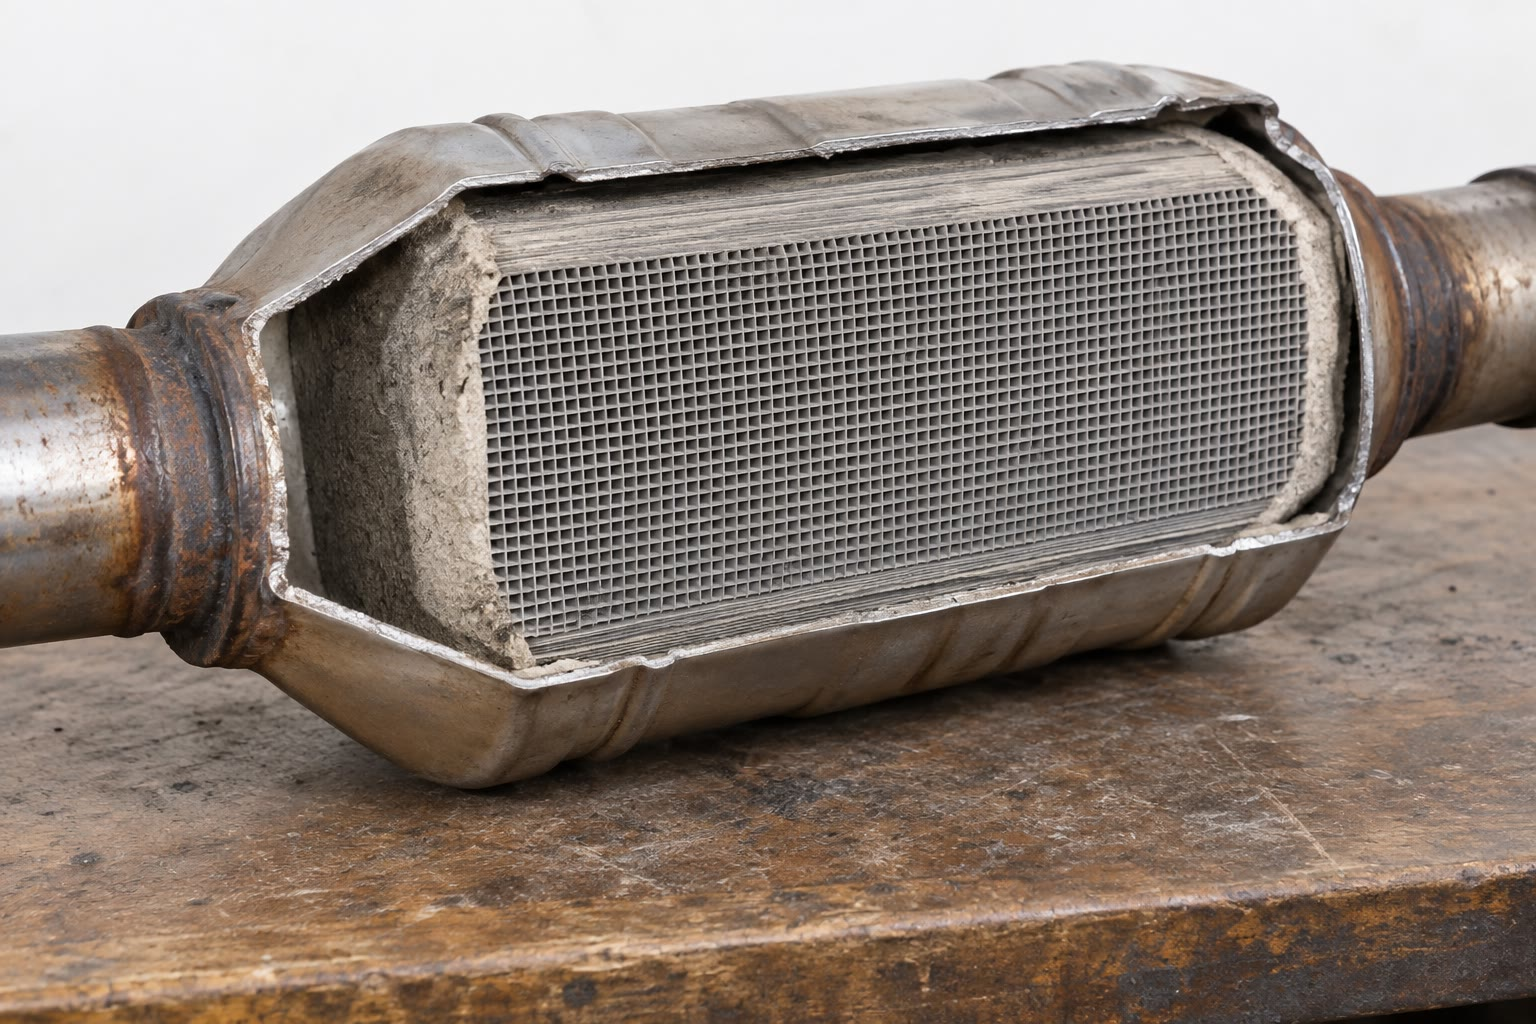
\includegraphics[width=0.45\linewidth]{images/book1/ai/g12-catalytic-converter.jpg}

{\small खोलकर काटा गया एक \omterm{def:g12:catalysis:catalyst}{उत्प्रेरक} परिवर्तक: मधुकोश वाला भीतरी भाग।}
\end{omfigure}

\begin{history}[हाबर, बॉश और अमोनिया]
% ledger: haber:T, haber:p, nh3:world-2024
बीसवीं शताब्दी के आरंभ में रसायनज्ञ फ़्रिट्ज़ हाबर ने खोजा कि
लौह-आधारित \omterm{def:g12:catalysis:catalyst}{उत्प्रेरक} पर \omterm{def:g4:air-a-mixture-of-gases:air}{वायु} की नाइट्रोजन को हाइड्रोजन से कैसे जोड़ा जाए,
\ce{N2 + 3H2 -> 2NH3}, और इंजीनियर कार्ल
बॉश ने इसे एक औद्योगिक प्रक्रम में बदल दिया। यह आज भी 400
से \qty{500}{\celsius} और 150 से \qty{250}{atm} पर चलता है। 2024 में विश्व ने
लगभग 15 करोड़ टन नाइट्रोजन वाली अमोनिया बनाई, जिसका अधिकांश
उर्वरकों के लिए था: हम जो भोजन खाते हैं, उसकी नाइट्रोजन का बड़ा हिस्सा
ऐसे ही \omterm{def:g12:catalysis:catalyst}{उत्प्रेरक} से होकर गुज़रा है।
\end{history}

\section{एंज़ाइम}

\begin{definition}[एंज़ाइम]\label{def:g12:catalysis:enzyme}
\emph{एंज़ाइम}\index{एंज़ाइम} किसी सजीव द्वारा बनाया गया वह प्रोटीन है
जो उसके रसायन की किसी एक अभिक्रिया को उत्प्रेरित करता है। एंज़ाइम अत्यंत दक्ष
और अत्यंत विशिष्ट होते हैं: हर एक केवल कुछ ही \omterm{def:g7:atoms-and-molecules:molecule}{अणुओं} पर फ़िट होता है, और वे
ताप और अम्लता के एक संकरे परास में सबसे अच्छा काम करते हैं।
\end{definition}

\begin{example}[कैटालेज़]\label{ex:g12:catalysis:catalase}
हाइड्रोजन परॉक्साइड कोशिकाओं में उप-उत्पाद के रूप में बनता है, और उनके लिए
हानिकारक है। रक्त, यकृत और अनेक पादप ऊतकों में मौजूद \omterm{def:g12:catalysis:enzyme}{एंज़ाइम} कैटालेज़
उसे अत्यधिक तेज़ी से पानी और ऑक्सीजन में अपघटित करता है: यही
छिले हुए घुटने पर, या कच्चे आलू की फाँक पर, बनने वाला झाग है। उबला आलू
कोई झाग नहीं देता: गरम करने ने \omterm{def:g12:catalysis:enzyme}{एंज़ाइम} की आकृति नष्ट कर दी है।
\end{example}

\begin{omfigure}
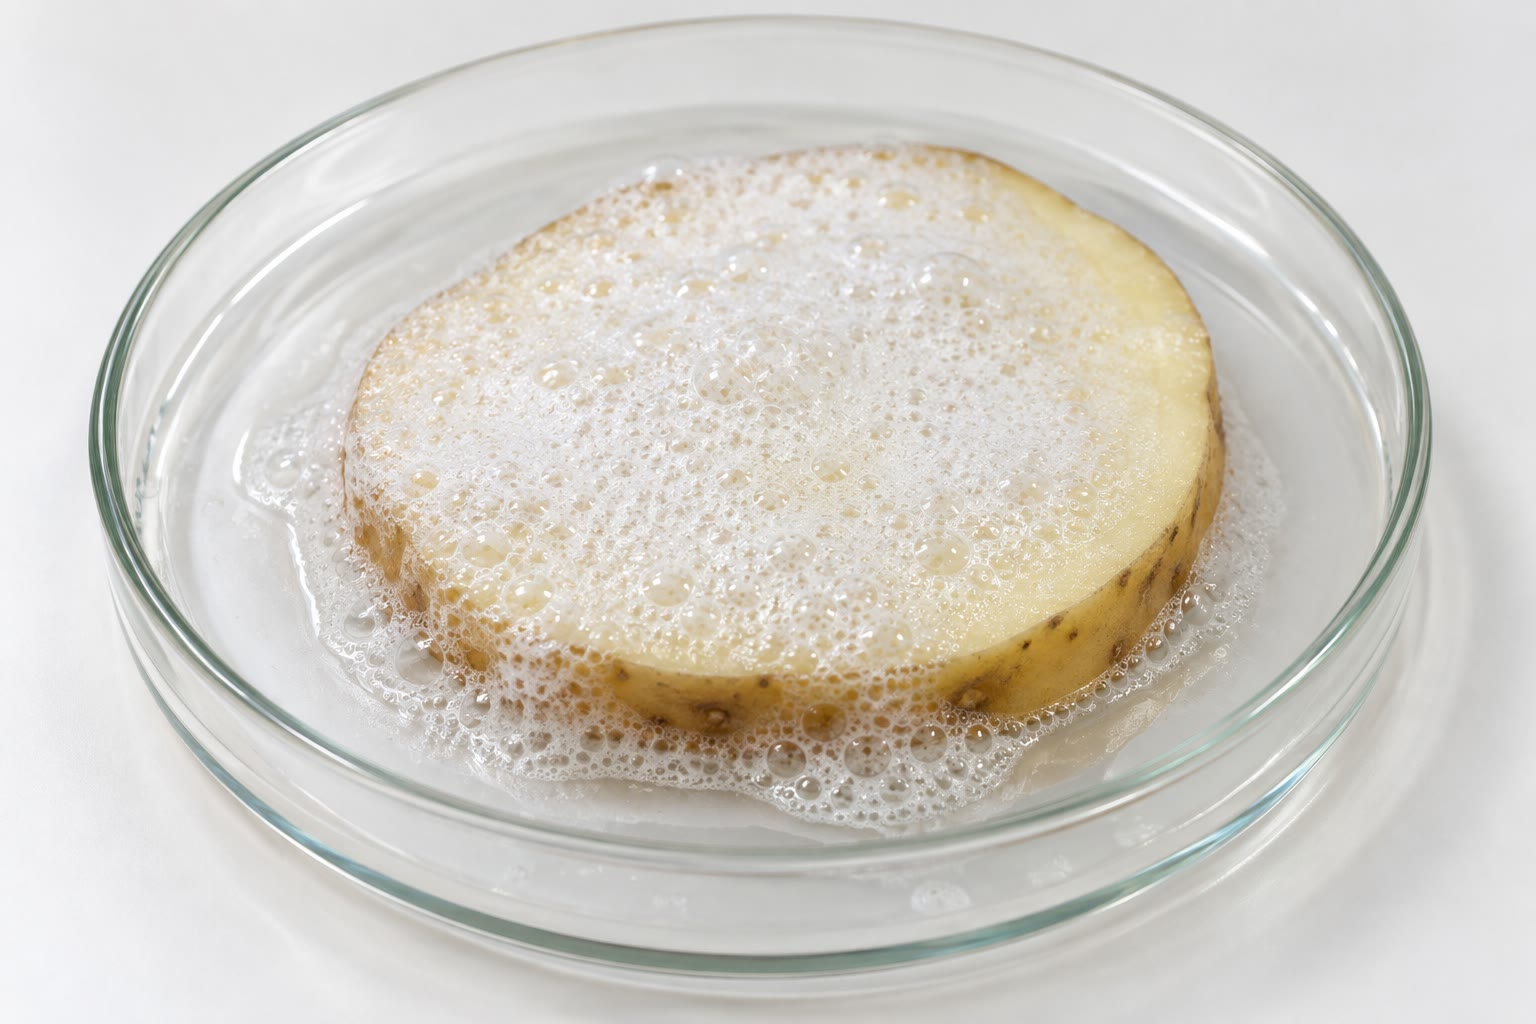
\includegraphics[width=0.45\linewidth]{images/book1/ai/g12-potato-peroxide.jpg}

{\small कच्चे आलू की फाँक पर हाइड्रोजन परॉक्साइड: काम करता हुआ कैटालेज़।}
\end{omfigure}

\section{वरणात्मकता}

\begin{definition}[वरणात्मक उत्प्रेरक]\label{def:g12:catalysis:selective}
जब वही \omterm{def:g7:chemical-reactions:reactant}{अभिकारक} कई अभिक्रियाएँ दे सकते हों, तो \emph{वरणात्मक
उत्प्रेरक}\index{वरणात्मक उत्प्रेरक} उनमें से एक को दूसरों की तुलना में
कहीं अधिक तेज़ करता है, और इस तरह तय करता है कि कौन-से उत्पाद बनेंगे।
\end{definition}

\begin{example}[एथेनॉल की दो नियतियाँ]\label{ex:g12:catalysis:ethanol}
ऐलुमिना के ऊपर से गुज़ारी गई गरम एथेनॉल वाष्प पानी खोकर एथीन देती है,
\ce{C2H5OH -> C2H4 + H2O} (एक \omterm{def:g12:curly-arrows:categories}{विलोपन}); गरम ताँबे के ऊपर से गुज़ारने पर वह
हाइड्रोजन खोकर एथेनैल देती है, \ce{C2H5OH -> CH3CHO + H2}। वही
\omterm{def:g7:chemical-reactions:reactant}{अभिकारक}, दो \omterm{def:g12:catalysis:catalyst}{उत्प्रेरक}, दो उत्पाद।
\end{example}

\begin{remark}[उद्योग और जीवन उत्प्रेरकों पर चलते हैं]\label{rem:g12:catalysis:everywhere}
रासायनिक उद्योग के अधिकांश उत्पाद, \omterm{def:g4:what-a-fire-needs:fuel}{ईंधनों} से लेकर \omterm{def:g8:plastics:plastic}{प्लास्टिक} और
उर्वरकों तक, \omterm{def:g12:catalysis:catalyst}{उत्प्रेरकों} से बनते हैं; अधिक सक्रिय या अधिक
\omterm{def:g12:catalysis:selective}{वरणात्मक उत्प्रेरक} खोजने से ऊर्जा और अपशिष्ट बचते हैं। किसी सजीव
कोशिका की हर अभिक्रिया किसी \omterm{def:g12:catalysis:enzyme}{एंज़ाइम} द्वारा उत्प्रेरित होती है।
\end{remark}

\begin{safety}{\ghs[0.82cm]{GHS03}\ghs[0.82cm]{GHS05}\ghs[0.82cm]{GHS07}}
% ledger: ghs:H2O2
सांद्र हाइड्रोजन परॉक्साइड एक प्रबल \omterm{def:g11:redox:oxidant}{ऑक्सीकारक} है जो आग को बढ़ा सकता है,
त्वचा और आँखों को जलाता है, और निगलने पर हानिकारक है। प्रयोगशाला के तनु
विलयनों के लिए भी चश्मा और दस्ताने चाहिए;
अपघटन से ऑक्सीजन निकलती है, इसलिए यह कभी बंद पात्र में नहीं किया जाता।
\end{safety}

\section{अभ्यास}


\begin{exercise}[$\star$]\label{exo:g12:catalysis:1}
आयोडाइड \omterm{def:g9:ions:ion}{आयनों} द्वारा उत्प्रेरित हाइड्रोजन परॉक्साइड के अपघटन में कौन-सी
स्पीशीज़ \omterm{def:g7:chemical-reactions:reactant}{अभिकारक} हैं, कौन-सी उत्पाद, कौन-सी \omterm{def:g12:catalysis:catalyst}{उत्प्रेरक} है, कौन-सी
मध्यवर्ती है?
\end{exercise}

\begin{exercise}[$\star$]\label{exo:g12:catalysis:2}
समांगी या \omterm{def:g12:catalysis:homogeneous}{विषमांगी उत्प्रेरण}: हाइड्रोजन परॉक्साइड विलयन में आयोडाइड \omterm{def:g9:ions:ion}{आयन};
\omterm{def:g12:catalysis:catalyst}{उत्प्रेरक} परिवर्तक में प्लैटिनम; अमोनिया \omterm{def:g10:synthesis-yield:synthesis}{संश्लेषण} में लोहा;
हाइड्रोजन परॉक्साइड विलयन में आयरन(III) \omterm{def:g9:ions:ion}{आयन}?
\end{exercise}

\begin{exercise}[$\star$]\label{exo:g12:catalysis:3}
ऊर्जा-रूपरेखाओं पर किस रास्ते की बाधा ऊँची है? क्या दोनों रास्तों पर
आरंभिक और अंतिम ऊर्जाएँ एक ही हैं? उत्पादों के लिए इसका क्या अर्थ
है?
\end{exercise}

\begin{exercise}[$\star$]\label{exo:g12:catalysis:4}
\omterm{def:g12:catalysis:catalyst}{उत्प्रेरक} किसी अभिक्रिया के समग्र समीकरण में क्यों दिखाई नहीं देता?
\end{exercise}

\begin{exercise}[$\star$]\label{exo:g12:catalysis:5}
उद्योग के ठोस \omterm{def:g12:catalysis:catalyst}{उत्प्रेरक} बारीक चूर्ण के रूप में या सरंध्र आधारों पर पतली
परतों के रूप में क्यों इस्तेमाल किए जाते हैं?
\end{exercise}

\begin{exercise}[$\star\star$]\label{exo:g12:catalysis:6}
हाइड्रोजन परॉक्साइड के आयरन(III)-उत्प्रेरित अपघटन के दोनों चरणों को जोड़िए,
और दिखाइए कि आयरन \omterm{def:g9:ions:ion}{आयन} और हाइड्रोजन \omterm{def:g9:ions:ion}{आयन} कट जाते हैं।
\end{exercise}

\begin{exercise}[$\star\star$]\label{exo:g12:catalysis:7}
निकली ऑक्सीजन के वक्र पढ़िए। हर प्रयोग को अंतिम आयतन का आधा
निकालने में कितना समय लगता है? \omterm{def:g12:catalysis:catalyst}{उत्प्रेरक} इसे किस गुणक से
छोटा कर देता है?
\end{exercise}

\begin{exercise}[$\star\star$]\label{exo:g12:catalysis:8}
\omterm{def:g12:catalysis:catalyst}{उत्प्रेरक} परिवर्तक वाली कारों में सीसायुक्त पेट्रोल इस्तेमाल नहीं किया जाता: सीसा
प्लैटिनम पर जम जाता है और वहीं रहता है। समझाइए कि यह परिवर्तक को क्यों बर्बाद कर देता है,
यद्यपि सामान्य अभिक्रिया में प्लैटिनम खपता नहीं।
\end{exercise}

\begin{exercise}[$\star\star$]\label{exo:g12:catalysis:9}
एक छात्रा 10, 25, 37, 60 और \qty{80}{\celsius} पर हाइड्रोजन
परॉक्साइड में आलू की फाँकों द्वारा बनाया गया झाग मापती है: झाग
लगभग \qty{37}{\celsius} तक बढ़ता है, फिर घटता है, और \qty{80}{\celsius} पर लगभग
गायब हो जाता है। वक्र के दोनों भागों को समझाइए।
\end{exercise}

\begin{exercise}[$\star\star$]\label{exo:g12:catalysis:10}
\omterm{def:g12:catalysis:catalyst}{उत्प्रेरक} परिवर्तक में कार्बन मोनोऑक्साइड और नाइट्रोजन मोनोऑक्साइड के बीच
अभिक्रिया का समीकरण लिखिए, और जाँचिए कि वह संतुलित है।
दोनों प्रदूषक एक साथ क्यों हट जाते हैं?
\end{exercise}

\begin{exercise}[$\star\star$]\label{exo:g12:catalysis:11}
हाइड्रोजन परॉक्साइड विलयन के \qty{10.0}{mL} पूर्ण अपघटन पर \qty{20}{\celsius} पर
\qty{72}{mL} ऑक्सीजन देते हैं। ऑक्सीजन की मात्रा
($V_m = \qty{24.1}{L/mol}$) निकालिए, फिर विलयन में
हाइड्रोजन परॉक्साइड की सांद्रता।
\end{exercise}

\begin{exercise}[$\star\star\star$]\label{exo:g12:catalysis:12}
ऐलुमिना के ऊपर से गुज़ारी गई एथेनॉल वाष्प एथीन देती है; ताँबे के ऊपर से वह
एथेनैल देती है। दोनों समीकरण लिखिए, पहले की श्रेणी बताइए, और
समझाइए कि \omterm{def:g12:catalysis:selective}{वरणात्मक उत्प्रेरक} क्या है।
\end{exercise}

\begin{exercise}[$\star\star\star$]\label{exo:g12:catalysis:13}
एक \omterm{def:g12:catalysis:catalyst}{उत्प्रेरक} किसी अभिक्रिया को दस गुना तेज़ कर देता है। एक छात्र दावा करता है कि वह
दस गुना अधिक उत्पाद भी देता है। निकली ऑक्सीजन के वक्रों की मदद से
दावे को सुधारिए।
\end{exercise}

\begin{exercise}[$\star\star\star$]\label{exo:g12:catalysis:14}
कैटालेज़ का एक \omterm{def:g7:atoms-and-molecules:molecule}{अणु} प्रति सेकंड हाइड्रोजन परॉक्साइड के कुछ दस लाख
\omterm{def:g7:atoms-and-molecules:molecule}{अणुओं} को अपघटित करता है। प्रति सेकंड $\num{5e6}$ लेकर, एक \omterm{def:g12:catalysis:enzyme}{एंज़ाइम} \omterm{def:g7:atoms-and-molecules:molecule}{अणु} को
हाइड्रोजन परॉक्साइड का एक \omterm{def:g10:the-mole:amount}{मोल} अपघटित करने में कितना समय लगता है?
कितने \omterm{def:g12:catalysis:enzyme}{एंज़ाइम} \omterm{def:g7:atoms-and-molecules:molecule}{अणु} इसे एक सेकंड में कर देंगे? (परिमाण की कोटियों पर एक
गणना; दर अभ्यास के लिए दिया गया आँकड़ा है।)
\end{exercise}

\begin{exercise}[$\star\star\star$]\label{exo:g12:catalysis:15}
% ledger: nh3:world-2024
2024 में विश्व ने अमोनिया में लगभग 15 करोड़ टन नाइट्रोजन बनाई।
यह अमोनिया का कितना द्रव्यमान है? डाइनाइट्रोजन की कितनी मात्रा संयोजित हुई?
\end{exercise}

\section{समस्या: नाई की दुकान का परॉक्साइड}

\begin{problem}[{सप्ताहांत समस्या --- ``20 आयतन'' वाले हाइड्रोजन परॉक्साइड की
सांद्रता क्या है?}]
\label{pb:g12:catalysis:1}
% ledger: const:Vm1, ghs:H2O2, aw:H, aw:O
बाल सँवारने वाले ``आयतनों'' में अंकित हाइड्रोजन परॉक्साइड विलयन इस्तेमाल करते हैं:
``20 आयतन'' वाला विलयन वह है जिसका \qty{1}{L} पूर्ण अपघटन पर \qty{20}{L}
ऑक्सीजन देता है, गैस को \qty{0}{\celsius} और सामान्य वायुमंडलीय दाब पर
मापकर, जहाँ गैस का एक \omterm{def:g10:the-mole:amount}{मोल}
\qty{22.4}{L} घेरता है।

\medskip
\noindent\textbf{भाग I --- अपघटन।}
\begin{enumerate}
  \item हाइड्रोजन परॉक्साइड के अपघटन का समीकरण लिखिए।
  \item क्या अपघटन एक \omterm{def:g11:redox:reaction}{अपचयोपचय अभिक्रिया} है? \omterm{def:g11:redox:oxidant}{ऑक्सीकारक} और
        \omterm{def:g11:redox:oxidant}{अपचायक} खोजिए (हाइड्रोजन परॉक्साइड दोनों है)।
  \item अभिक्रिया संभव होते हुए भी बोतल महीनों तक क्यों टिकी रहती है?
\end{enumerate}

\medskip
\noindent\textbf{भाग II --- ``20 आयतन'' का अर्थ।}
\begin{enumerate}[resume]
  \item विलयन का \qty{1}{L} ऑक्सीजन की कितनी मात्रा देता है?
  \item \qty{1}{L} में हाइड्रोजन परॉक्साइड की मात्रा निकालिए।
  \item \omterm{def:g10:concentration-and-dilution:molar-concentration}{मोलर सांद्रता} बताइए।
  \item हाइड्रोजन परॉक्साइड का \omterm{def:g10:the-mole:molar-mass}{मोलर द्रव्यमान} और \omterm{def:g10:concentration-and-dilution:mass-concentration}{द्रव्यमान
        सांद्रता} निकालिए।
  \item \omterm{def:g10:the-mole:amount}{मोल} प्रति लीटर में ``10 आयतन'' का क्या अर्थ होगा?
\end{enumerate}

\medskip
\noindent\textbf{भाग III --- दो \omterm{def:g12:catalysis:catalyst}{उत्प्रेरक}।}
\begin{enumerate}[resume]
  \item एक नमूने में रक्त की एक बूँद (कैटालेज़), और दूसरे में आयरन(III) क्लोराइड की कुछ बूँदें,
        मिलाई जाती हैं। हर एक कौन-सा \omterm{def:g12:catalysis:catalyst}{उत्प्रेरण} है?
  \item आयरन(III) \omterm{def:g12:catalysis:catalyst}{उत्प्रेरण} के दोनों चरण लिखिए और जाँचिए कि
        उनका योग अपघटन है।
  \item निकली ऑक्सीजन के वक्रों की मदद से वर्णन कीजिए कि \omterm{def:g12:catalysis:catalyst}{उत्प्रेरक} के साथ और उसके बिना
        ऑक्सीजन का आयतन कैसे बदलता है, और क्या वही
        रहता है।
  \item आयरन(III)-उत्प्रेरित नमूने का रंग अभिक्रिया के दौरान क्यों बदलता है
        और अंत में लौट आता है?
  \item उबला आलू विलयन में झाग क्यों नहीं बनाता?
\end{enumerate}

\medskip
\noindent\textbf{भाग IV --- बोतल।}
\begin{enumerate}[resume]
  \item \qty{100}{mL} की बोतल \qty{0}{\celsius} पर मापी गई ऑक्सीजन का
        कितना आयतन दे सकती है?
  \item \qty{20}{\celsius} ($V_m =
        \qty{24.1}{L/mol}$) पर यह कितना आयतन है?
  \item ऐसी बोतल के ढक्कन को गैस धीरे-धीरे निकलने क्यों देनी चाहिए?
  \item लंबे समय तक रखी एक बोतल का \omterm{def:g11:titration:titration}{अनुमापन} करने पर उसमें
        \qty{1.50}{mol/L} पाया जाता है। अब यह कितने ``आयतन'' है?
  \item हाइड्रोजन परॉक्साइड का कितना भाग अपघटित हो चुका है?
  \item अंतिम उत्तर बताइए: ``20 आयतन'' वाले हाइड्रोजन परॉक्साइड
        विलयन की \omterm{def:g10:concentration-and-dilution:molar-concentration}{मोलर सांद्रता} क्या है?
\end{enumerate}
\end{problem}
